\documentclass[11pt,a4paper]{article}
\usepackage[utf8]{inputenc}
\usepackage{amsmath}
\usepackage{pdflscape}
\usepackage{amsfonts}
\usepackage{float}
\usepackage{graphicx}
\usepackage{amssymb}
\usepackage{parskip}
\title{\vspace{-2.0cm} Assignment 1}
\author{Celina Ma, John Ngo, Omar Qureshi}
\begin{document}
\maketitle
\def\textfraction{.01}
\def\topfraction{.99}
\section*{Deliverable \#1}

Generally, the software development model is chosen in response to the circumstances of the software’s development. Our client is a real-world client – Professor Jason Donev, who is an individual and understandably has a busy schedule. He can meet up with us around once a week, but it would be difficult and unreasonable to remain in constant communication. There are difficulties for us as well as students going to classes on a set schedule, thus any method which requires constant client input and interaction on every aspect of development appears unsuitable. This difficulty eliminates the Scrum model, due to it being an agile model which requires such constant communication.

Next, we must consider our requirements, or lack there of. As we currently understand it, our client has a general trajectory as to what sort of software product he wants, but not the full specification of what exactly is desired down to the last detail. Furthermore, future improvement ideas have been discussed and thought of as early as the very beginning of the project, such as integrating a similar but not identical device – the Geiger counter. These facts strongly point away from incremental models, towards iterative models. 

Furthermore, we are all inexperienced in this project, not knowing the full details of what we might need to learn to complete this project, thus we cannot easily and evenly divide up the project – ruling out the concurrent model directly. The waterfall model requires a more intensive discussion with the client period before dropping off the radar and just building the software, where the first half might demand more attention than can be reasonably provided and the latter half squanders our ability to contact him for more questions, clarifications, and demonstrations of prototypes. As such, the Waterfall model is no fit either.

Phased release also suffers from the same intense requirements gathering phase needed in the beginning, and the rolling out of the releases do not actually factor in input from the client, again squandering a major advantage of being able to meet with and discuss the project with our client. As such, phased release is also not a reasonable model.

We are now left with the Spiral and Opportunistic models. Of these, the Opportunistic model doesn’t factor in client communication, and is not a clear and reliable software development plan for any external client or larger project. The scope of our project is not so small that the opportunistic model can work, since an app with multiple parts is much larger than projects suited for opportunistic, such as brief Computer Science class assignments or small segments of code. This leaves the Spiral model.

The spiral model’s quick cycles complete with risk assessment, planning and development stages appear to fit perfectly for this setup. In these brief meetings, we can gather requirements from our client and demonstrate the project as it currently stands; as it is an iterative model we can accommodate for changes in the project requirements and for future upgrades. As such, Spiral is a near perfect fit for our situation, and as such will be used.

\section*{Deliverable \#2}

\subsection*{2-1: Functional Requrements (FRs)}

\vskip 3mm

1. "The app must be able to receive data from the muon detector."

This app must be able to communicate with the external piece of hardware in order to meet the criteria given by the client. 

\vskip 6mm

2. "The app must be able to display a 'live' reading from the muon detector."

Along with receiving input from the detector, it then must be able to display the stream of values outputted by the detector onto the phone. 

\vskip 6mm

3. "The app must be able to average out the last 10 readings when pressing the 'get reading' button"

While a live reading is displayed, the 'get reading' button takes a snapshot of the readings average and displays a constant value underneath the live readings. 

\vskip 6mm
4. "The app must be able to record the averaged  'get readings' in a table." 

After pressing the 'get reading' button, the value is averaged and stored into a table that is accessible in another part/menu of the application.

\vskip 6mm
5. "The app must be able to export out the saved data to a computer so that further data interpretation and processing can be performed."

The client has specified that the readings once in tabled format must be able to export (via .csv for example) to another computer. This would progress the learning experiences of future students who want to work with the data more comfortably once it has been collected via the phone.  


\subsection*{2-2: Non Functional Requirements (NFRs)}

1. "The app should present the readings with two significant digits."

This allows the user to experience a non cluttered UI, removing unnecessary information. This NFR would fall under the usability. 

\vskip 4mm

2. "The app should record the readings by making a smooth visual animation."

A transition animation is often desired to express user action in a clearer way. This NFR would fall under the usability category. 

\vskip 4mm

3. "The app should record the readings within 0.5s after pressing the 'get reading' button."

This ensures the user doesn't have to wait an unusually large amount of time to get the reading. It also stops the user from getting frustrated and pressing the button again needlessly. This NFR would fall under the response time category. 
\vskip 4mm
4. "The app should emit a feedback sound when the user presses the ‘get reading button’" 

Giving the user direct confirmation of their action being applied is helpful and again stops user from pressing the button unnecessarily. This NFR would fall under the usability category.

\vskip 4mm
5. "The app should present a message if the muon detector is connected or not."

This makes sure that a precondition of using the app is met, which is having the miniUSB cable plugged into the phone and detector. This NFR would fall under the learnability/usability category. 


\newpage

\section*{Deliverable \#3}

\subsection*{3-1: Choosing User Stories Vs Use Cases}

After considering both use cases and user stories, we conclude that the user stories method is a better way to represent the systems requirements for our project. Just as with the selection of our software process model, this comes from consideration of our circumstances compared to the strengths and weaknesses of each model.

The largest, most important draw of the user stories model is that it is extremely simple and to the point. Its structure, where a given user wants to do something for a given reason, is very, very close to how our client expresses what he wants out of the software, and as such is extremely attractive. Along with the emphasis on action and reason, user stories allow for the communication of overarching requirements goals as opposed to more nitty-gritty details, which fits with the iterative model of development we have chosen, since iterative models work towards a general end goal but don’t care about details at each stage.

The largest, most important draw of the use cases model is that done correctly, it can map out the structure of the very application needed, at least on some level. However, this backbone given and its greater emphasis on specific details compared to user stories does not lend it quite as well to an iterative model; and furthermore, it is more technically designed than user stories, which are closer to natural language. As such, while not a terrible alternative, it just doesn’t provide nearly as many advantages as with user stories.

Therefore, we have selected user stories to represent our system requirements.


\subsection*{3-2: User Stories}

The three core functional requirements that the user (in our case Professor Donev) needs to accomplish are as follows: connect muon detector to phone, view muon detector data and save data from muon detector to a log. As such, three corresponding story cards are created; 

\newpage


\begin{figure}[h]
  \centering
  
      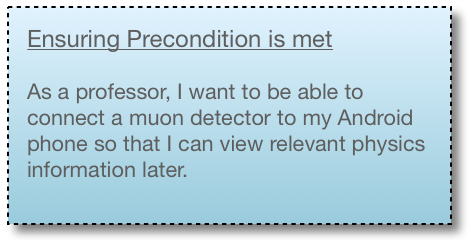
\includegraphics[width=0.7\textwidth]{storycard1.png}
  
\end{figure}

\begin{figure}[h]
  \centering
  
      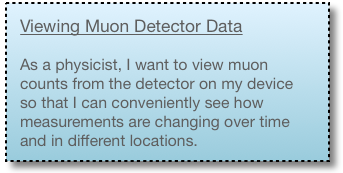
\includegraphics[width=0.7\textwidth]{storycard2.png}
     
  
\end{figure}

\begin{figure}[h]
  \centering
  
      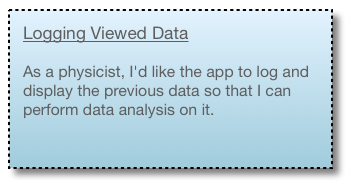
\includegraphics[width=0.7\textwidth]{storycard3.png}
      \caption{Individual story cards are first created to document core requirements, upon which further cards will be used to document how a user goes about accomplishing those tasks}
  
\end{figure}


\subsection*{3-3: Story Map}

With the use of the user story cards above, a collage/story map can be created that details further on how a user can interact with the app to accomplish their requirements. The story map can be viewed on the next landscape page;

\newpage
\begin{landscape}
\begin{figure}[h]
  \centering
  \vspace*{-2cm} \hspace*{-0.5cm}
      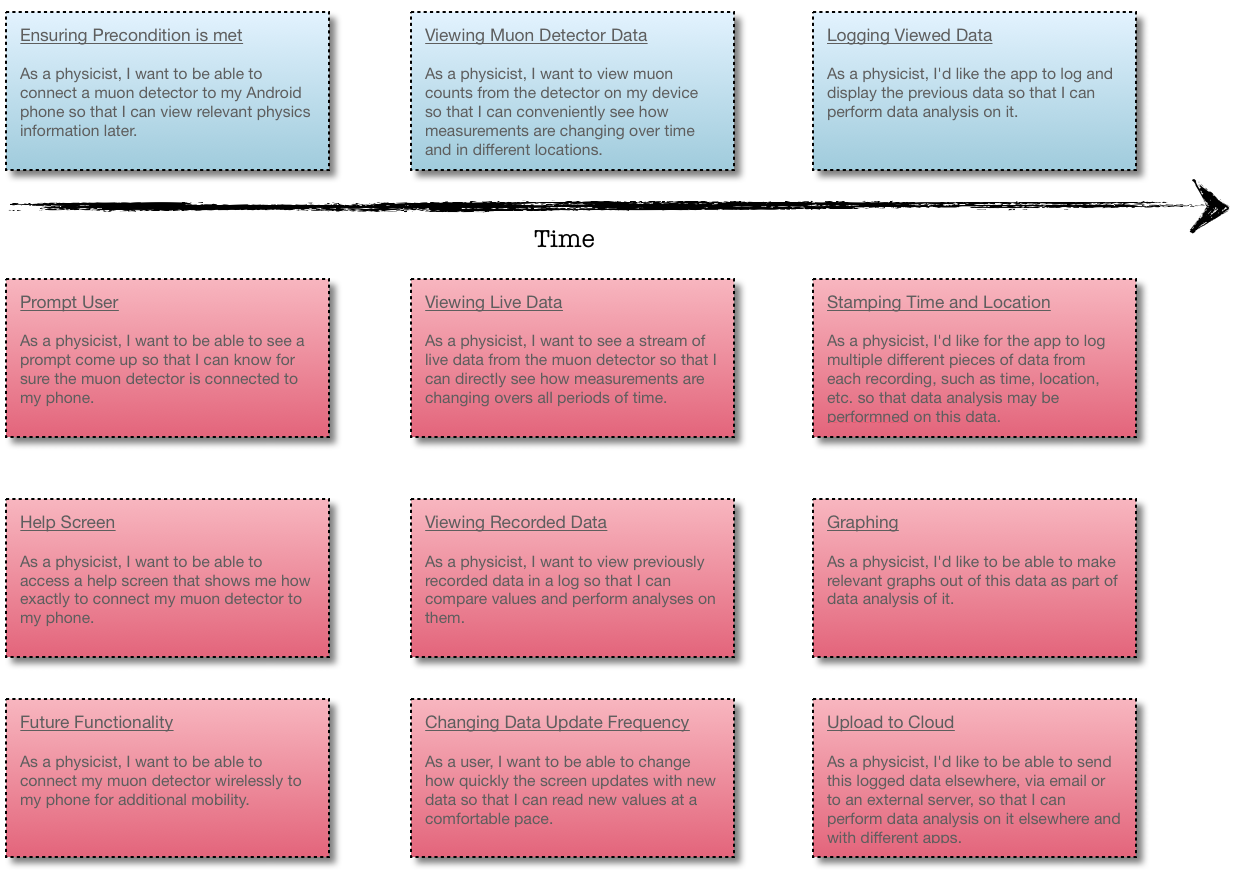
\includegraphics[width=2.0\textwidth]{storymap.png}
      \caption{A story map is used to organize requirements in order of priority and to illustrate how user interacts with app}
  
\end{figure}
\end{landscape}

\section*{Deliverable \#4}
\subsection*{4-1: Overview Sketches}
\bigskip
\begin{figure}[h]
  \centering
      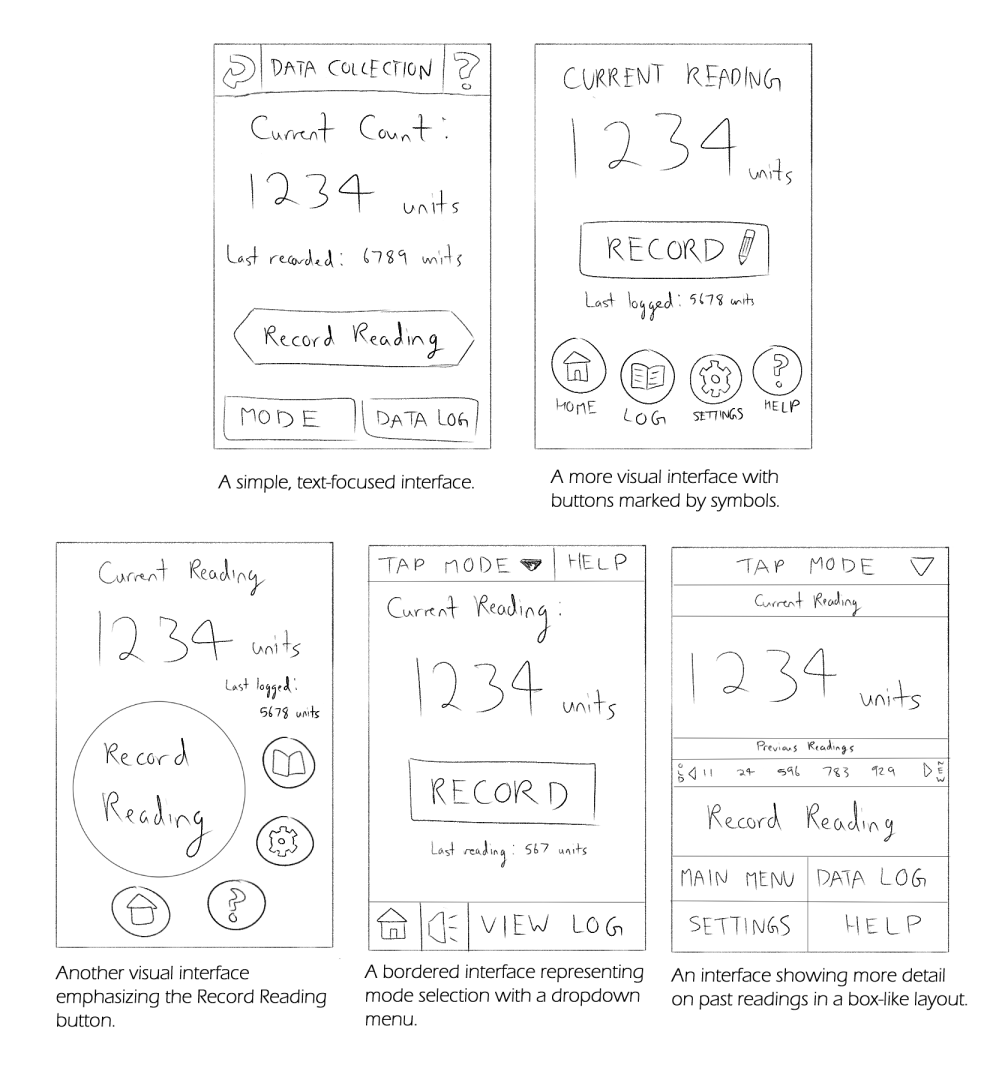
\includegraphics[width=1.1\textwidth]{overviewsketches.png}
  \caption{A variety of design approaches for the recording screen}
\end{figure}

\newpage
\subsubsection*{Why We Chose Sketch A}

We chose sketch A to elaborate on due to its clarity and emphasis on the most important aspects of this screen. The main buttons the user would interact with (Record, Mode and Data Log) are large and displayed clearly. Compared to sketches B and C, which have smaller icons that the user may accidentally mis-press, the interface of A is more focused on what is important to the user. This is key to enhancing the intuitiveness of the app. Sketch D emphasizes similar points to sketch A, but the mode selection button is somewhat less obvious in this design. Although sketch E shows more information about Previous Readings than the other sketches, it is too cluttered; additionally, that information is repeated in the Data Log screen in more detail, so it is not needed for the Data Collection screen. Thus, our main reason for choosing sketch A was its relative simplicity and correctly emphasized functions compared to the other designs.

\subsection*{4-2: Elaborating Sketches}
\def\textfraction{.01}
\def\topfraction{.99}
\bigskip
\begin{figure}[b!]
  \centering
  \hspace*{-1cm}
  \renewcommand{\textfraction}{0.05} 
      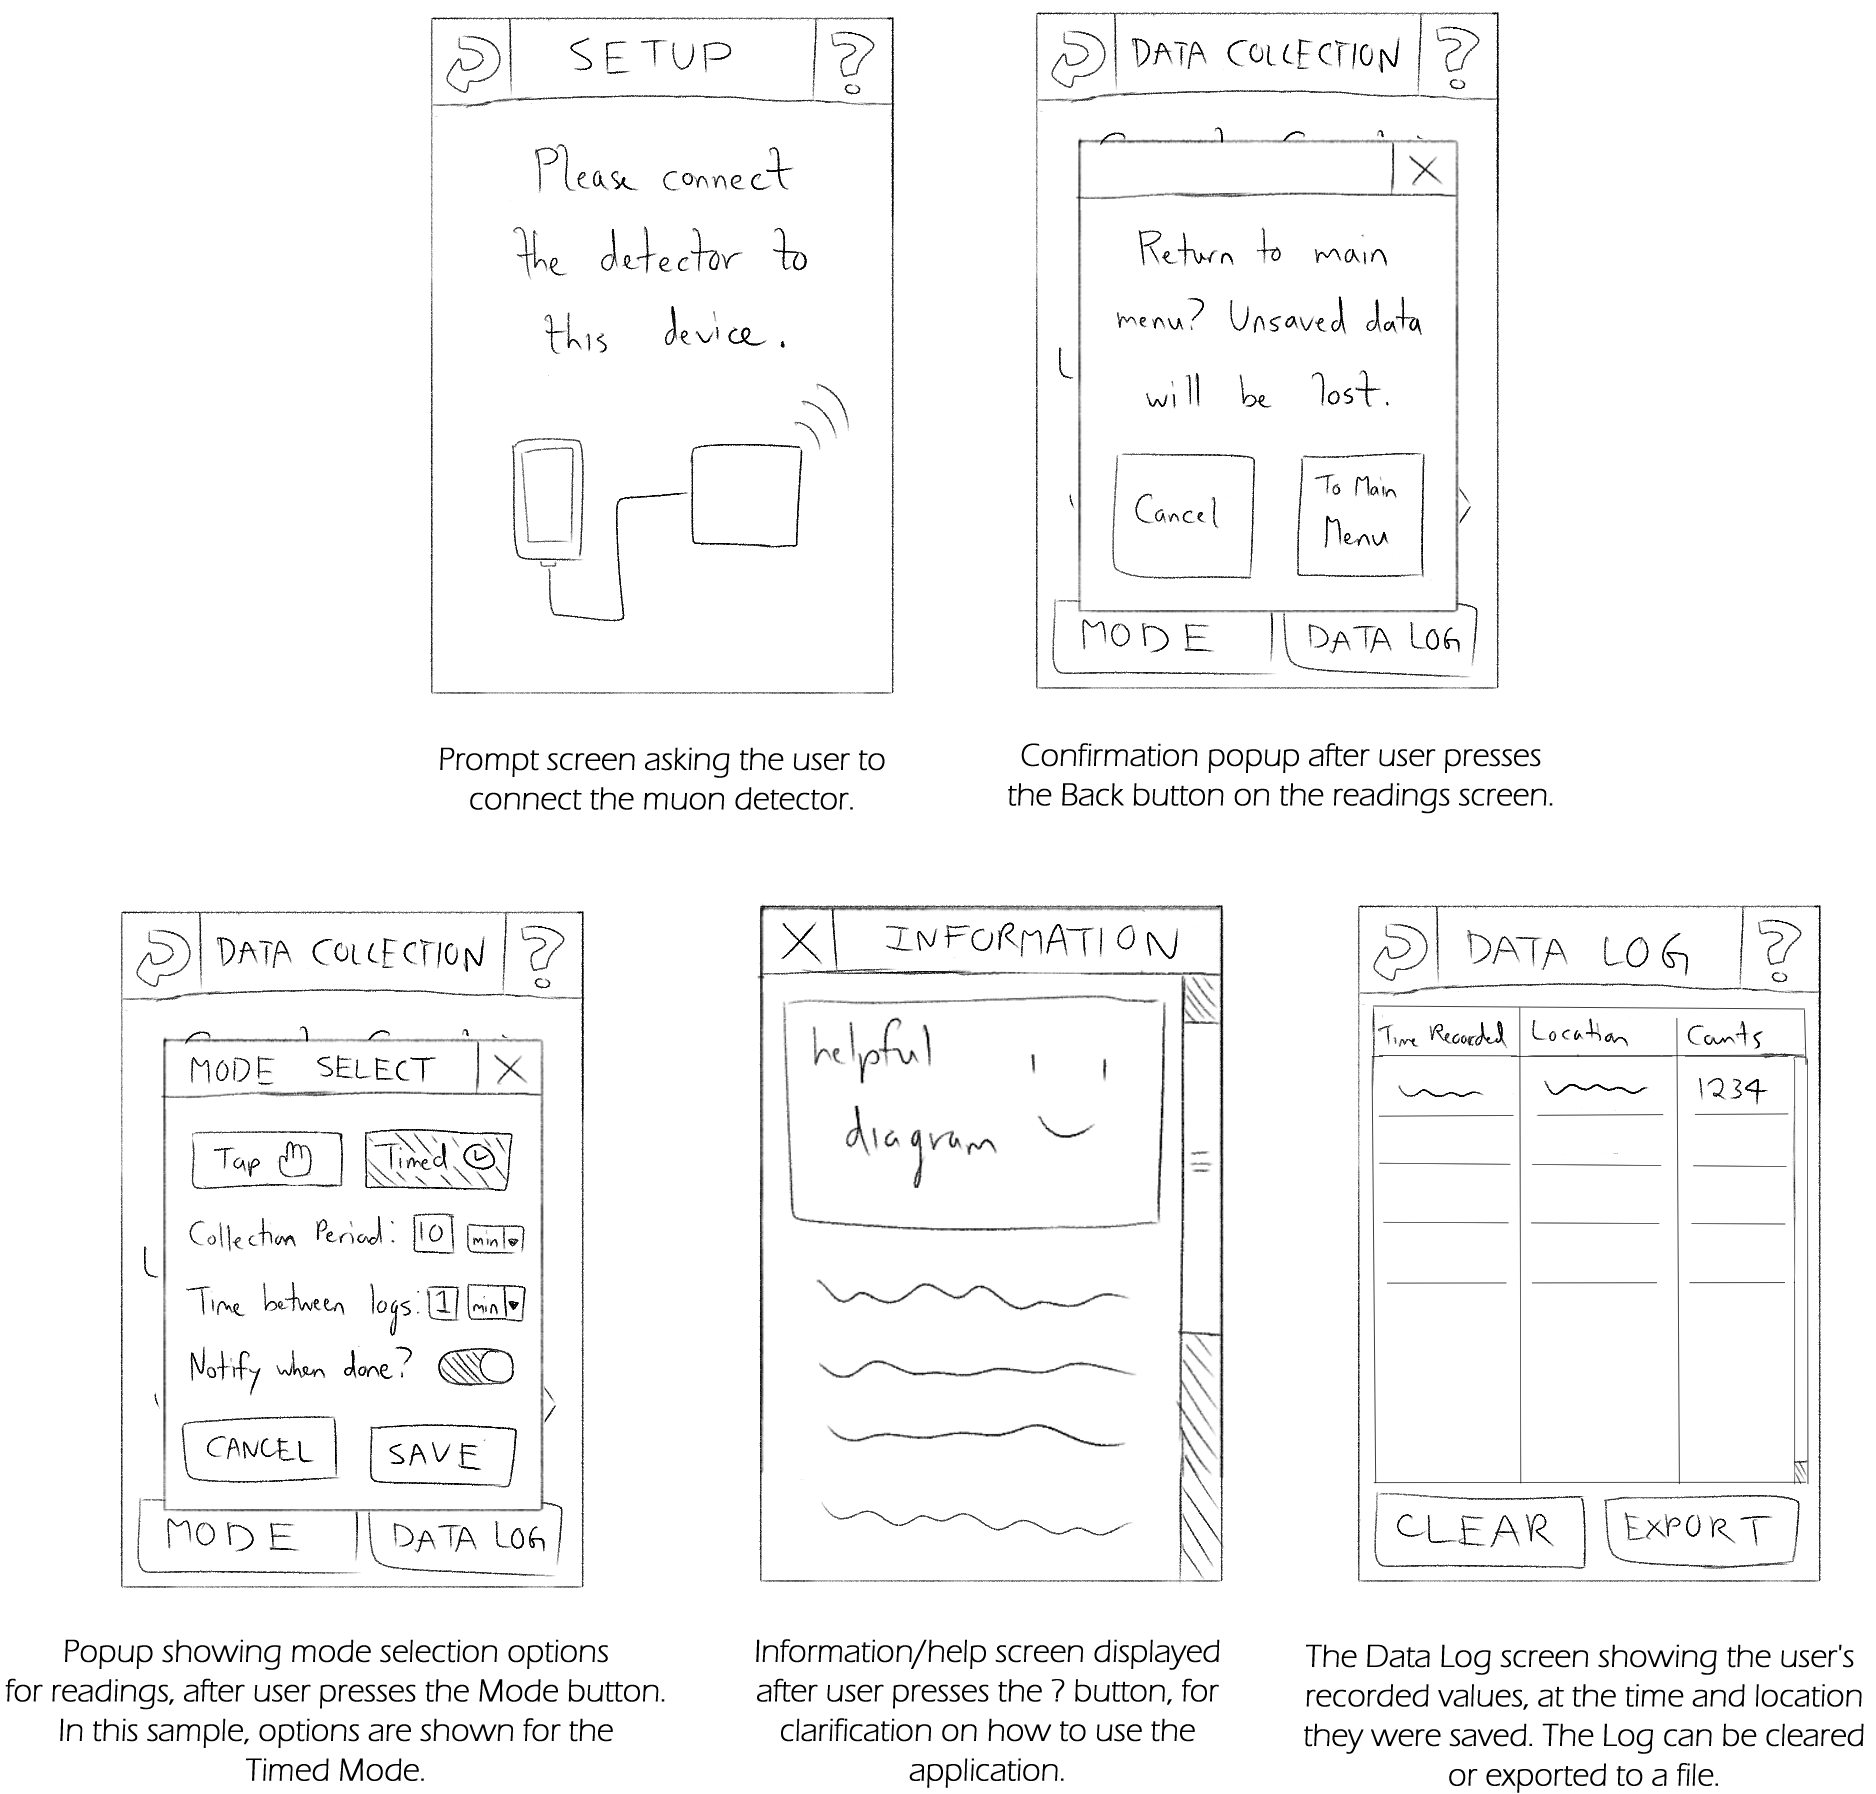
\includegraphics[width=0.84\textwidth]{elaboratingsketches.png}
  \caption{Extended sketches for other parts of the apps UI screens}
\end{figure}

\newpage
\subsection*{4-3: Storyboard Sketches}

\bigskip
\begin{figure}[h]
  \centering
  \hspace*{-0.5cm}
      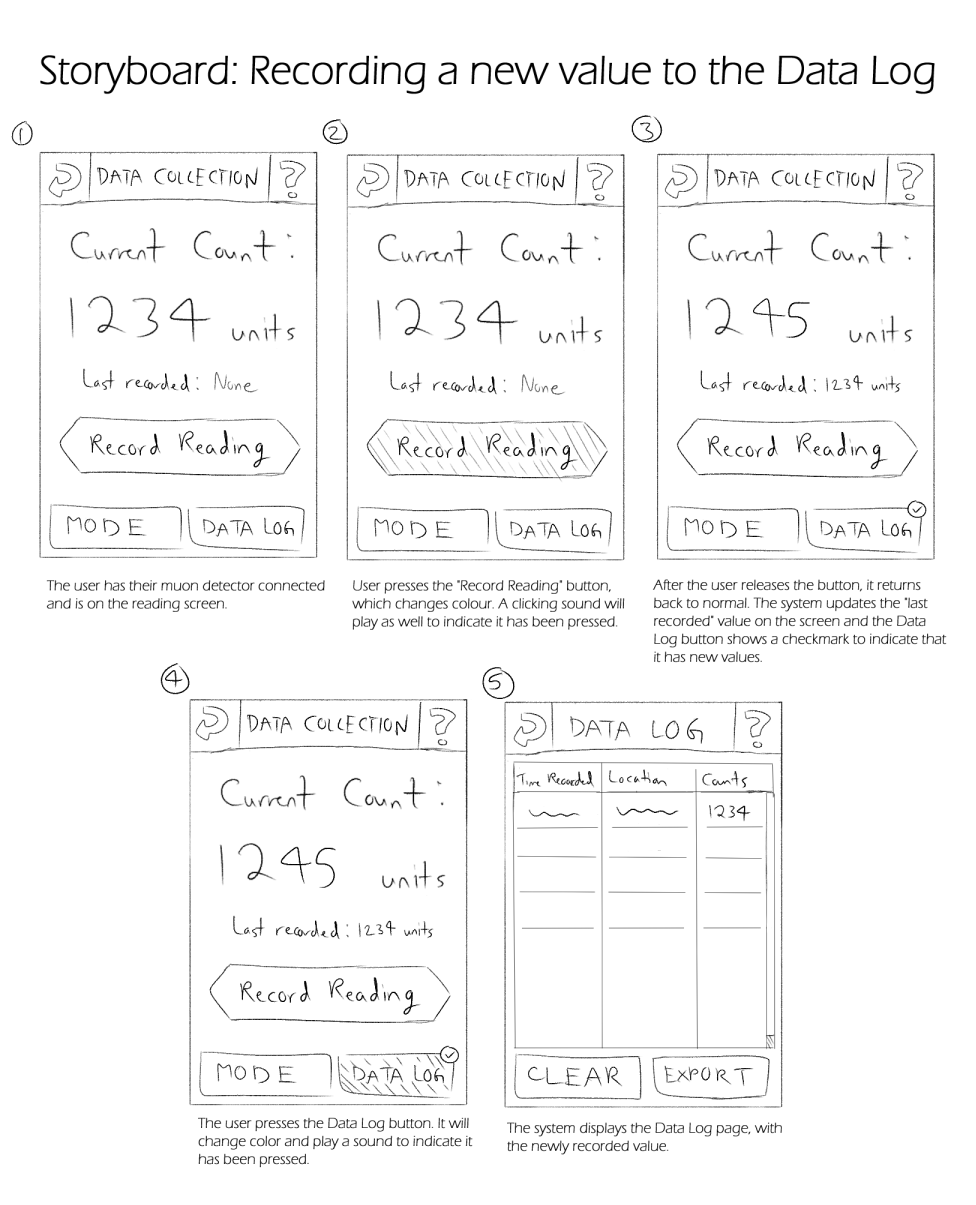
\includegraphics[width=1.15\textwidth]{storyboard.png}
  \caption{The recording screen responding to user input}
\end{figure}

\newpage
\subsection*{4-4: Wizard of Oz Demo Video}

Demo videos can be viewed at the following links:


\subsection*{4-5: Requirements Change}

When generating overview sketches for part 4-1, we had to consider what aspects of the Data Collection screen were most important for satisfying our initial requirements. All the sketches have similarities, such as having the live reading be the focus of the screen (FR \#2). However, they emphasized some different points, and we had to choose which design seemed most intuitive to use. For example, we considered if a settings button allowing the user to turn feedback sounds on/off (NFR \#4) was necessary on this screen, or if it was better suited for the main menu. As for the elaborating sketches, they were mainly based on our functional requirements (FR \#1 Collection Prompt; FR \#4 Data Log).  Deciding how the reading screen should be connected to other parts of the app was helpful for planning user navigation.

When storyboarding, we again focused on improving usability of the app. Along with playing a sound when the user presses the "get reading" button (NFR \#4), we added visual cues to indicate a successful recording. In this case, we changed the colour of the button and placed a checkmark symbol on the Data Log. So, the storyboarding process was helpful for generating more visual feedback to the user. This step was also useful for estimating how convenient it is to perform a key task in our interface (recording a value to the log).

The most helpful prototyping technique for adjusting our requirements was the Wizard of Oz video. Allowing Dr. Donev to directly interact with our paper prototype resulted in a great amount of feedback. We realized the discrepancies between our current design and what our client considered important. For example, we emphasized a constant, live stream of data (FR \#2), but Dr. Donev explained that we should only begin displaying data after pressing the record button. Rather than averaging readings (FR \#3), the application should function more like a counter over some time interval. He also introduced other requirements that we had not thought about before, like having the user indicate if they are indoors or outdoors when taking measurements. By discussing requirements and revising them with our client, we gained a much clearer image of how our application should work.



\newpage
\section*{Deliverable \#5}

Our project first began with John consulting us about a program an external client, Dr. Donev, might need. We agreed and this led to John emailing Dr. Donev to confirm the project. The following emails show the first steps in the project; 
\bigskip
\begin{figure}[h]
  \centering
      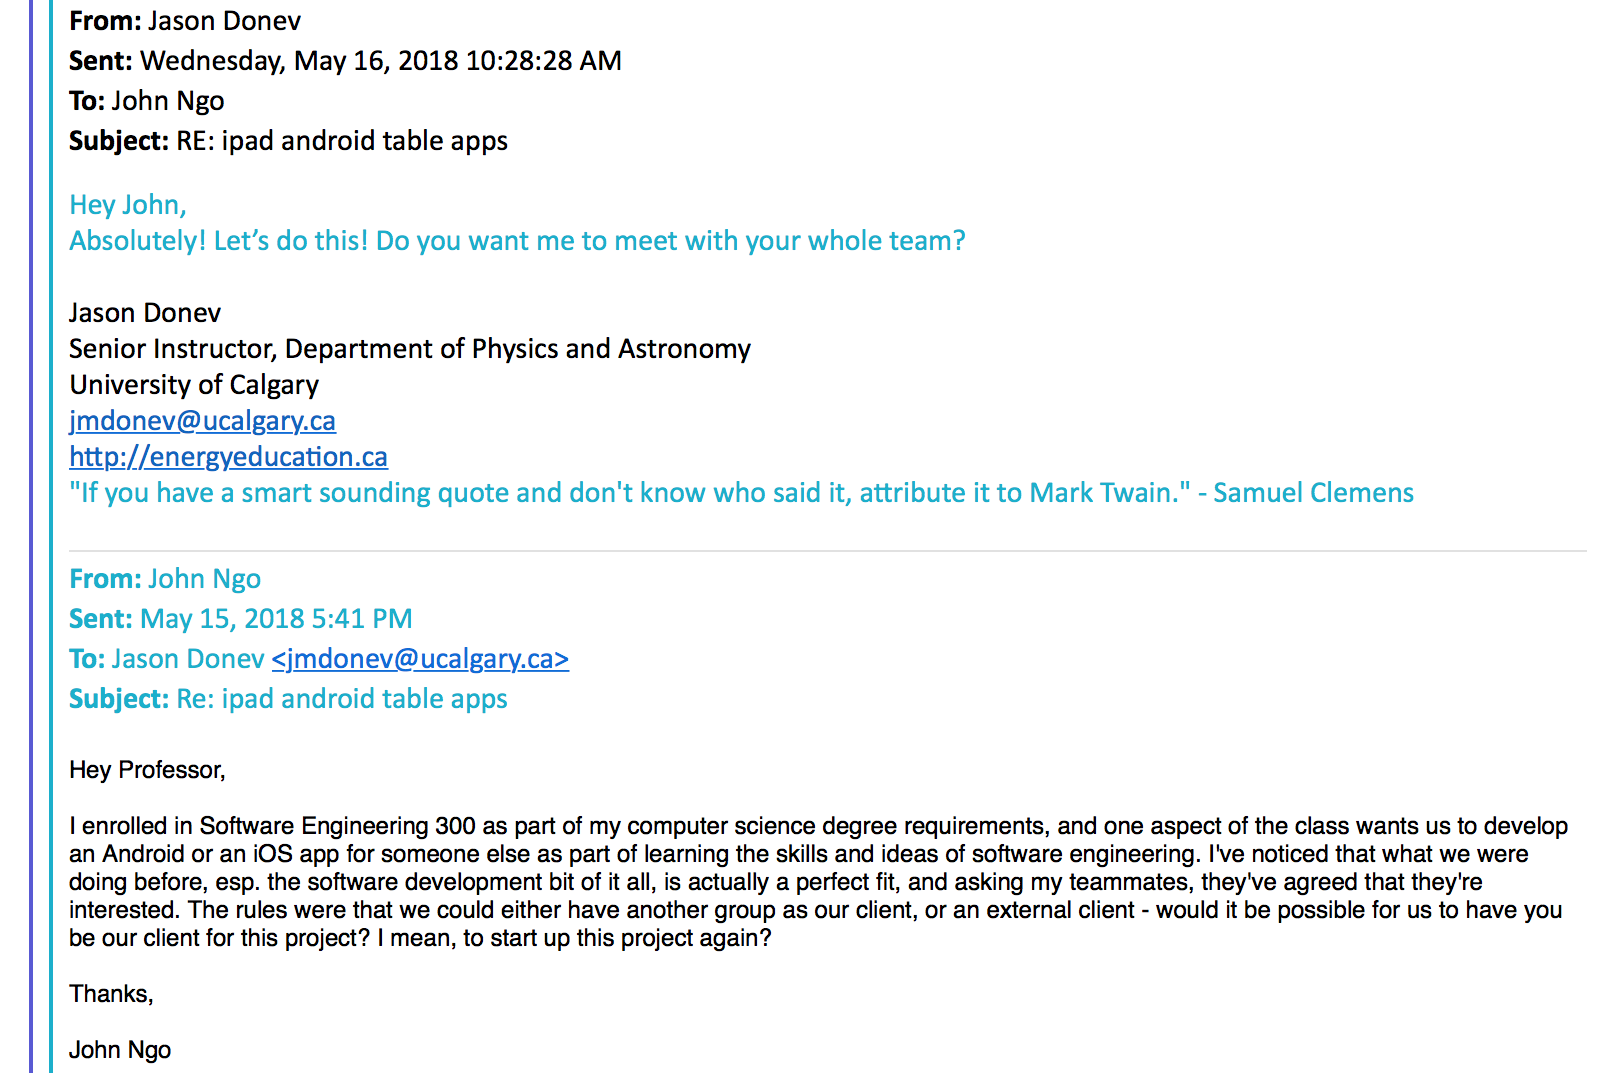
\includegraphics[width=1.1\textwidth]{1.png}
  \caption{Initial exchange of emails to get the project started}
\end{figure}

\newpage
Once the project was confirmed, Dr. Donev and John chatted on the phone to go over some project specifications very briefly. John told us a little about the app requirements such as it needing to communicate with an external piece of hardware. After some discussions of our own, we then met with Dr. Donev as a group after confirming a time;


\bigskip
\begin{figure}[h]
  \centering
      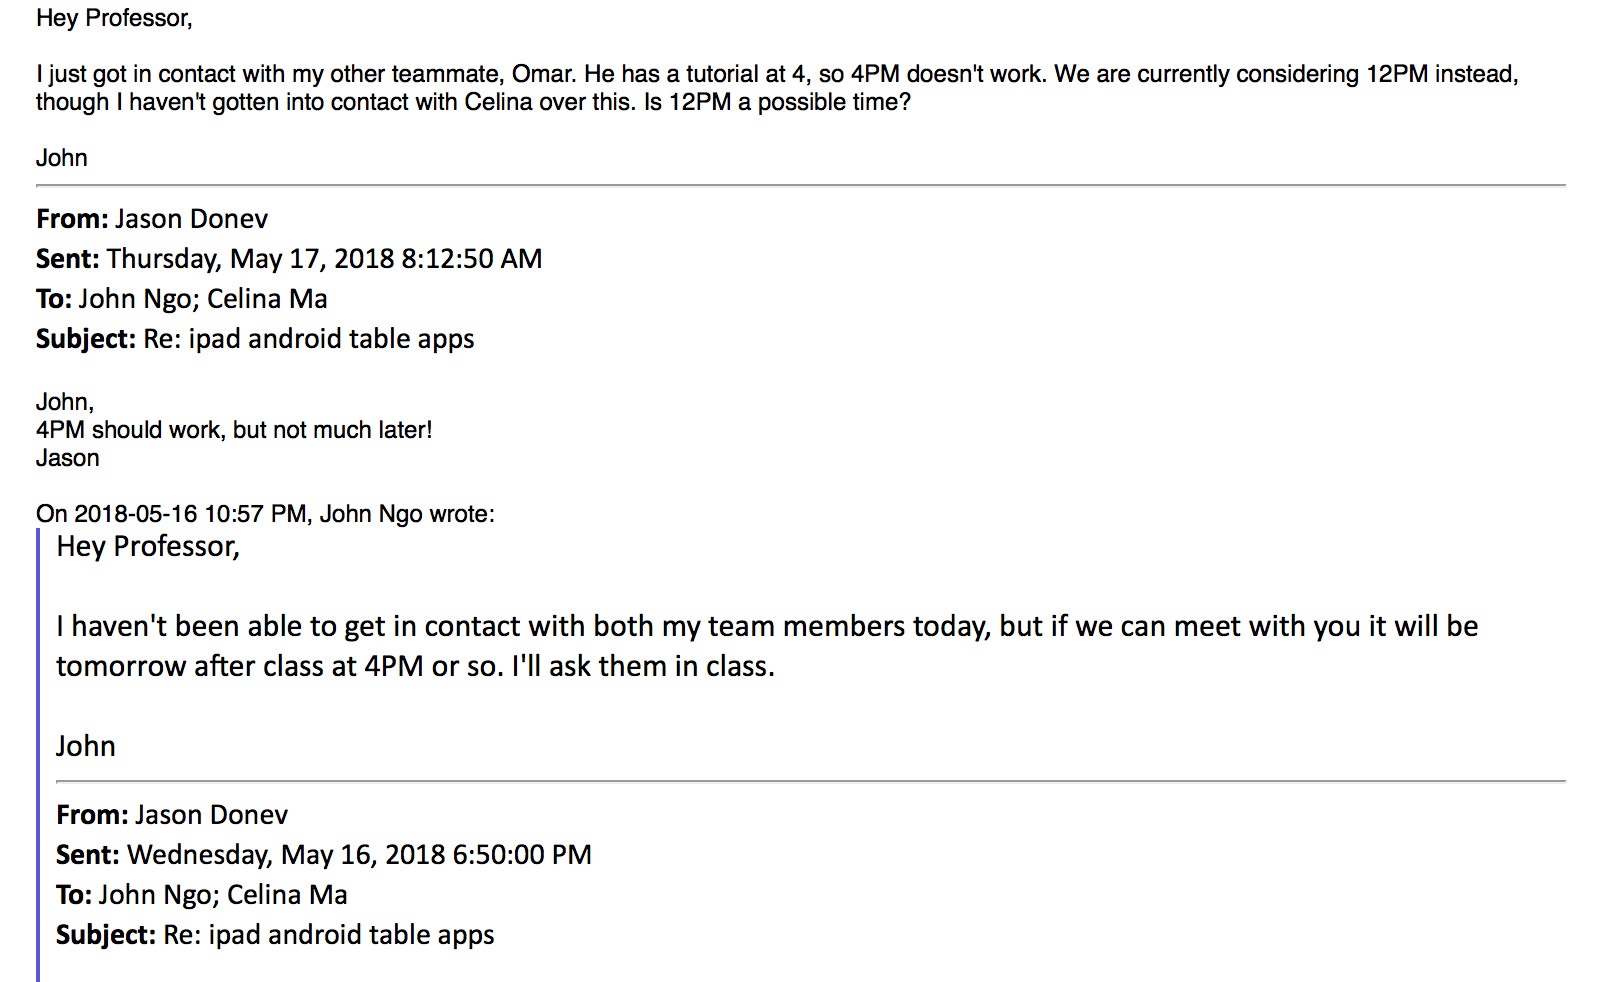
\includegraphics[width=1.1\textwidth]{3.png}

  \caption{Setting up a stand up meeting with Dr. Donev as a group}
\end{figure}


During this stand up meeting, we focused solely on requirements and what was the applications intended purpose. Some of the major requirements that were deduced were displaying a reading of the muons and being able to record that reading for data processing.

Approximately two weeks after the initial consult, we met with Dr. Donev again with a low fidelity prototype. This was the meeting where we recorded our Wizard of Oz style demo. 


\end{document}